\documentclass[margin=1cm]{standalone}
\usepackage{tikz}
\usetikzlibrary{automata, positioning, calc}
\begin{document}
	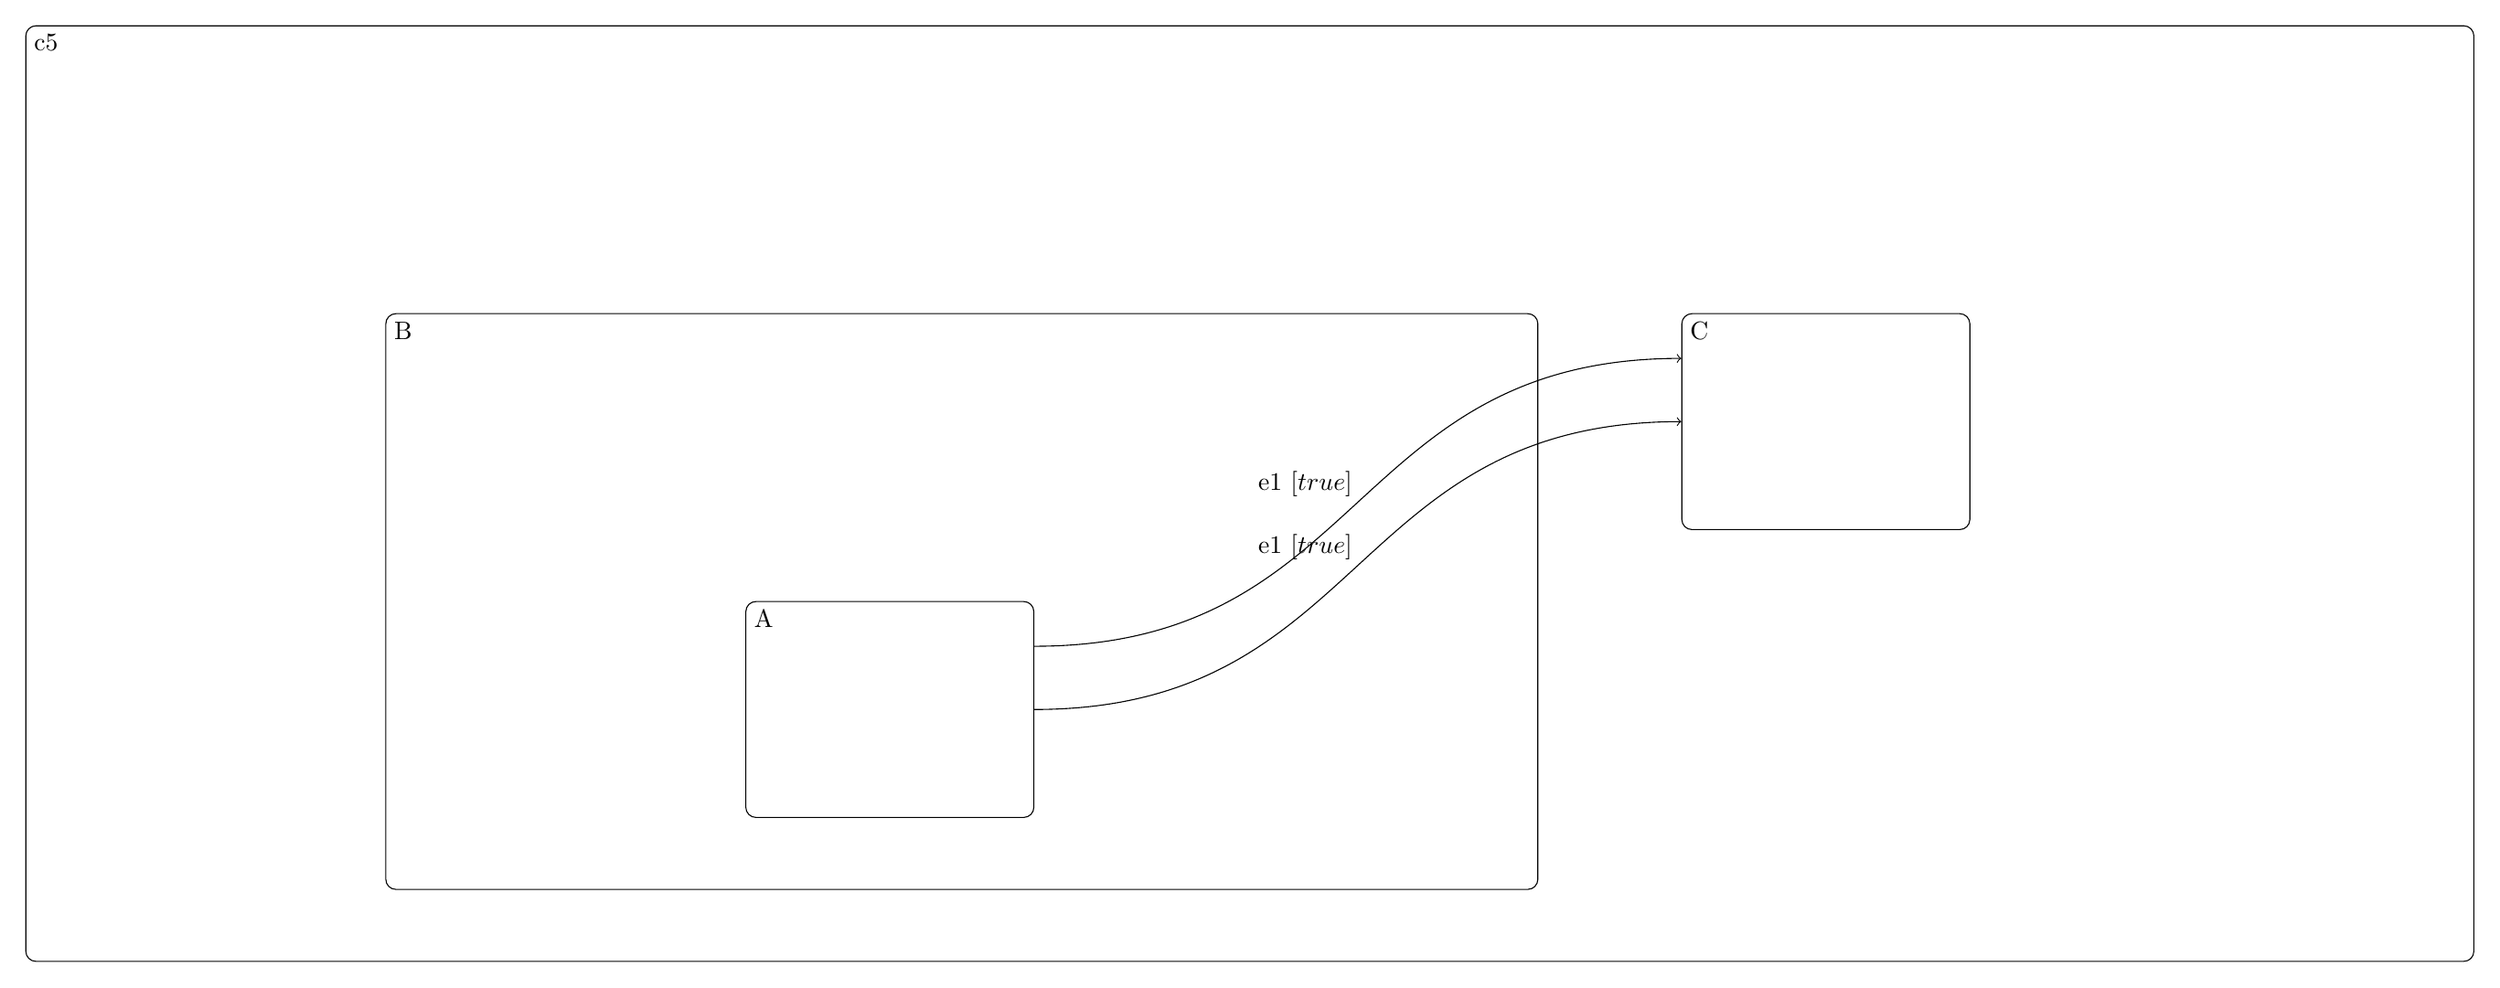
\begin{tikzpicture}[node distance=3cm, auto]
		\node[draw, rectangle, rounded corners, minimum width=34cm, minimum height=13cm, anchor=north west, label={[anchor=north west] north west:c5}] (c5) at (0, 0) {};
		\node[draw, rectangle, rounded corners, minimum width=16cm, minimum height=8cm, anchor=north west, label={[anchor=north west] north west:B}] (c5_B) at (5, -4) {};
		\node[draw, rectangle, rounded corners, minimum width=4cm, minimum height=3cm, anchor=north west, label={[anchor=north west] north west:A}] (c5_B_A) at (10, -8) {};
		\node[draw, rectangle, rounded corners, minimum width=4cm, minimum height=3cm, anchor=north west, label={[anchor=north west] north west:C}] (c5_C) at (23, -4) {};
		\draw[->] ($(c5_B_A.east) + (0, 0.0pt)$) to[out=0, in=180, looseness=1.2] node[pos=0.5, fill=white, inner sep=2pt] {e1 {$[true]$}} ($(c5_C.west) + (0, 0.0pt)$);
		\draw[->] ($(c5_B_A.east) + (0, 25.0pt)$) to[out=0, in=180, looseness=1.2] node[pos=0.5, fill=white, inner sep=2pt] {e1 {$[true]$}} ($(c5_C.west) + (0, 25.0pt)$);
	\end{tikzpicture}
\end{document}
